Contrarily from active enumeration, passive enumeration is a technique that does
not rely on explicit communication with a target system
\citep{cooperWhatDifferenceActive2020}. To perform a passive enumeration, a
network monitor tool such as Wireshark is often used.

\section{Connect to FTP}
\label{s:Connect-To-FTP}
The first part of the task is to connect to the ftp server and download the .pcap
file with all the captured network traffic.

\begin{figure}[ht]
  \centering
  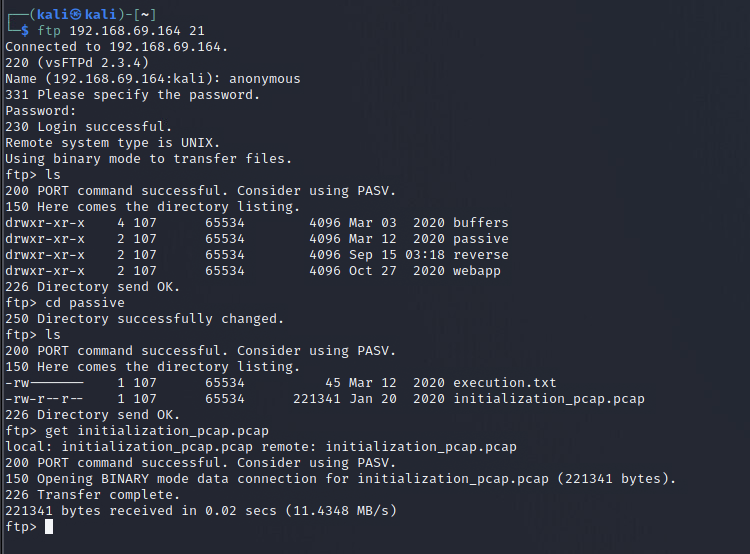
\includegraphics[width=0.7\textwidth]{figures/ftp-get-pcap}
  \caption{Connect to the FTP and get the .pcap file}
  \label{f:ftp-get-pcap}
\end{figure}

Now that the file has been downloaded, it can be found in the home (\~) directory
and we can start the analysis of the network traffic through Wireshark following the
tasks assigned to this lab.
\begin{figure}[ht]
  \centering
  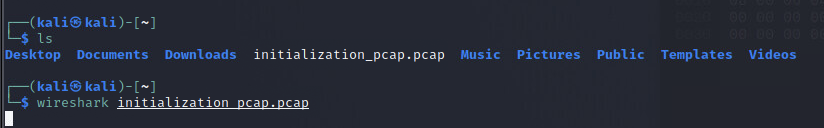
\includegraphics[width=0.7\textwidth]{figures/wireshark-pcap}
  \caption{Open .pcap with Wireshark}
  \label{f:wireshark-pcap}
\end{figure}

\section{Find unique IPv4 addresses}
\label{s:Find-Unique-IPv4-Addresses}
The first tasks asks to find the unique IPs that are stored and captured.
We can achieve that through the top menu, selecting statistics and IPv4 addresses.
The result is shown in the figure below.
\begin{figure}[H]
  \centering
  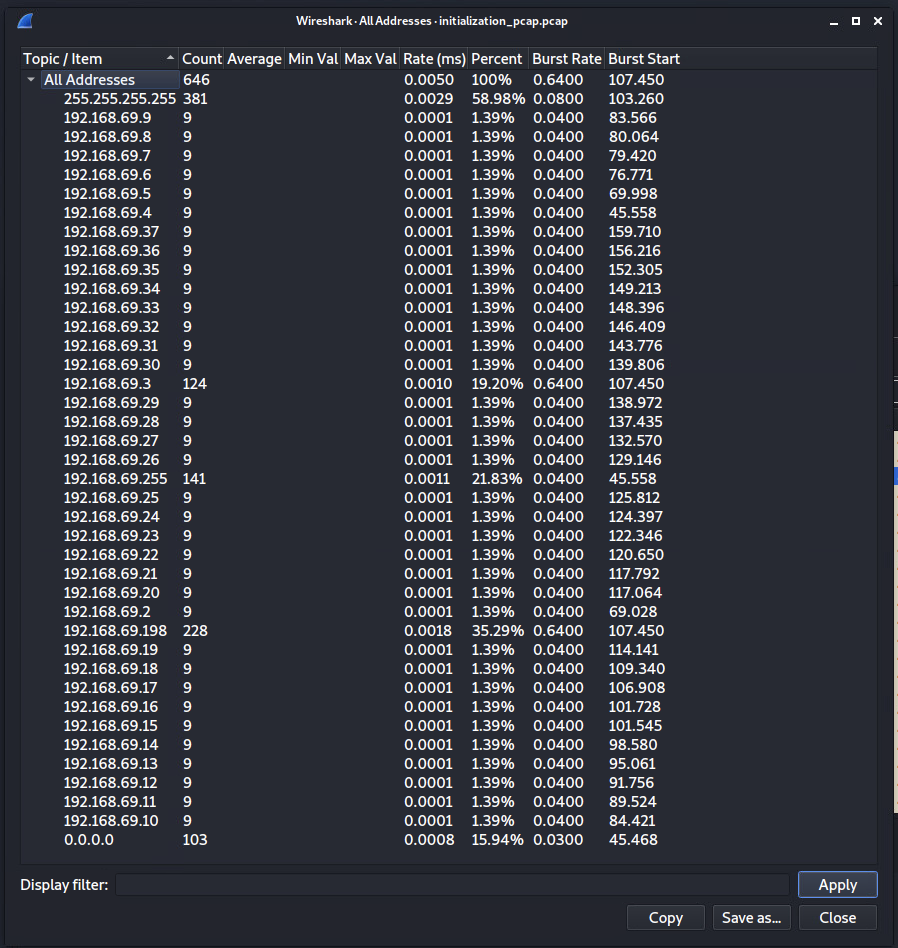
\includegraphics[width=0.7\textwidth]{figures/unique-ipv4-addresses}
  \caption{Unique IPv4 addresses}
  \label{f:unique-ipv4-addresses}
\end{figure}

\section{Application-layer Protocols}
\label{s:Application-layer-Protocols}
The second task asks to find the application-layer protocols that are used in the
captured network traffic. This can be displayed using the Protocol Hierarchy command.
The result is shown in the figure below.
\begin{figure}[ht]
  \centering
  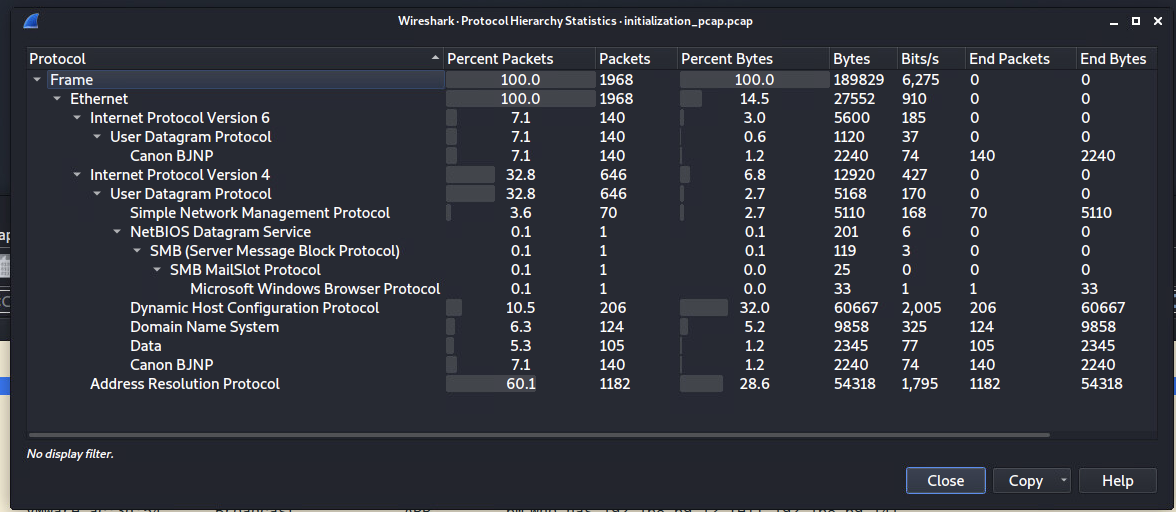
\includegraphics[width=1\textwidth]{figures/protocol-hierarchy}
  \caption{Protocol Hierarchy}
  \label{f:protocol-hierarchy}
\end{figure}

\section{Name of the protocols}
\label{s:Name-of-the-protocols}
The application-layer protocol are the following:

\begin{itemize}
  \item SNMP (Single Network Management Protocol): responsible for the management of
    network devices, allows the communication between them independently of their spec \citep{
    scarpatiWhatSimpleNetwork2020}.
  \item DNS (Domain Name System): responsible for the resolution of domain names to
    IP addresses \citep{insamApplicationLayerProtocol2020}.
  \item DHCP (Dynamic Host Configuration Protocol): responsible for the dynamic
    configuration of network devices. This protocol is used to automatically assign IPs
    to network devices \citep{ibmIBMDocs2021}.
  \item SMB (Server Message Block): responsible for the communication between
    shared devices such as printers on a network \citep{
    sheldonWhatServerMessage2020}.
\end{itemize}

\section{Network Diagram}
\label{s:Network-Diagram}
This task will allow us to have a visual representation of the analysis of the network.
Below the diagram with the active protocols and devices.

\begin{figure}[ht]
  \centering
  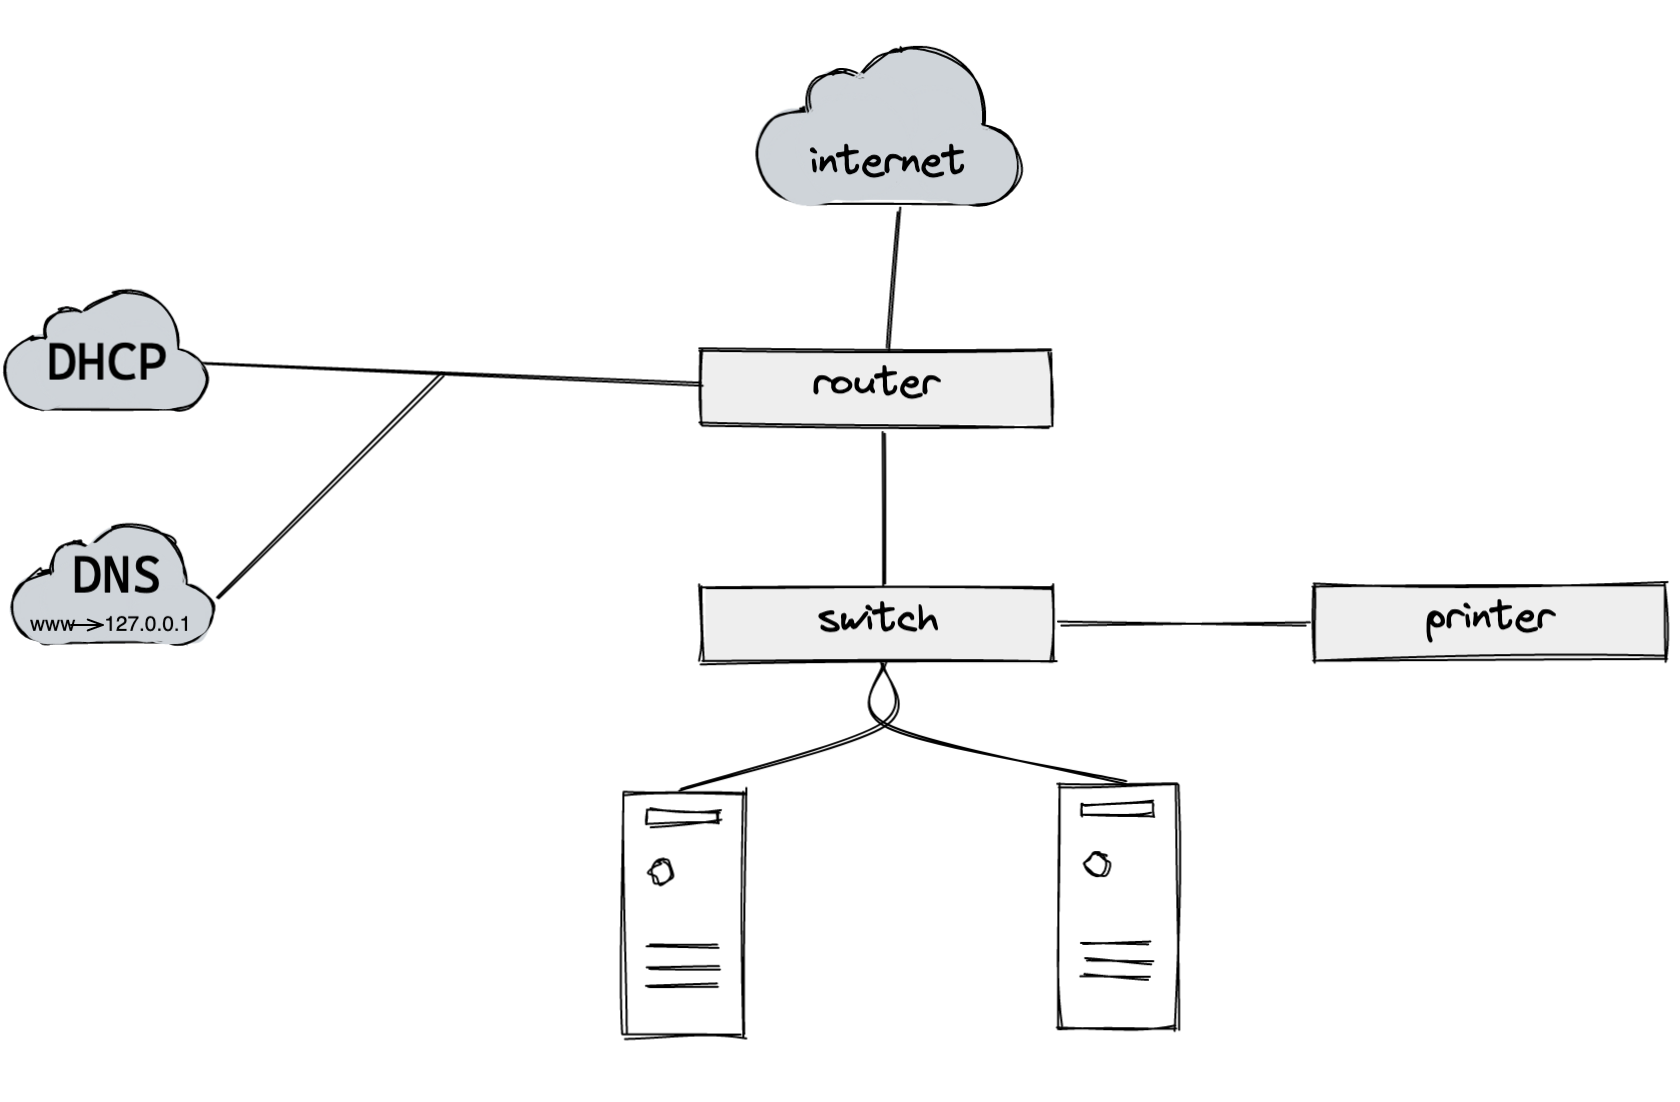
\includegraphics[width=1\textwidth]{figures/network-diagram}
  \caption{Network Diagram}
  \label{f:network-diagram}
\end{figure}

Following the explanation of the protocols, further analysis portrays the use of
internet protocol. The protocols in use are UDP, SNMP, DHCP and DNS, meaning
computers and shared devices on the network. We can also certify using a BJNP
protocol, meaning that the shared device on the network is a Canon printer.

\section{Discussion}
\label{s:Lab1-Discussion}
The network traffic analysis suggests that a user uses the shared device since
there is a BJNP protocol. There are also ACKs and NAKs portraying active
communication between the devices of the network.
Some of the UDP packets were broadcasting an std discovery all to find
all the services on the network.

\section{TCP Dump}
\label{s:TCP-Dump}
Following the instructions and the man page for the tcpdump command, I have been able
to reproduce a one liner to output a number of unique MAC addresses in the provided and previously
used .pcap file. Below a picture with the result.

\begin{figure}[ht]
  \centering
  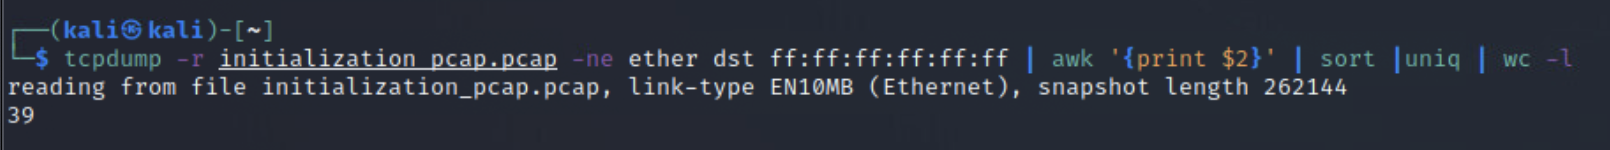
\includegraphics[width=1\textwidth]{figures/tcpdump}
  \caption{TCP Dump}
  \label{f:tcpdump}
\end{figure}

The flag \lstinline[language=bash]!-r! is used to read the file and the flag
\lstinline[language=bash]!-ne! before \lstinline[language=bash]!ether dst! looks
for ethernet destinations with the MAC address format specified right after it.
The command \lstinline[language=bash]!awk! is used to separate them while printing the
second argument to get the second column. It will then sort and check for unique
entries for then count everything with the last \lstinline[language=bash]!wc -l! command

\section{Reflection}
\label{s:Lab1-Reflection}
This has been a very fun lab. I have learned a lot more about Wireshark and how
to analyse a .pcap file. Even though I have never used
\lstinline[language=bash]!tcpdump!, there were manyexamples and exhaustive
official documentation.
